\subsection{Aufbau}
    Die meisten photovoltaischen Zellen haben den gleichen Grundaufbau
    und nur geringe Unterscheide wie das Muster der vorderen Kontakte
    oder die chemische Komposition der Anti-Reflexionschicht
    \cite{Wiki_SolarCell}.
    \begin{figure}[H]
        \centering
        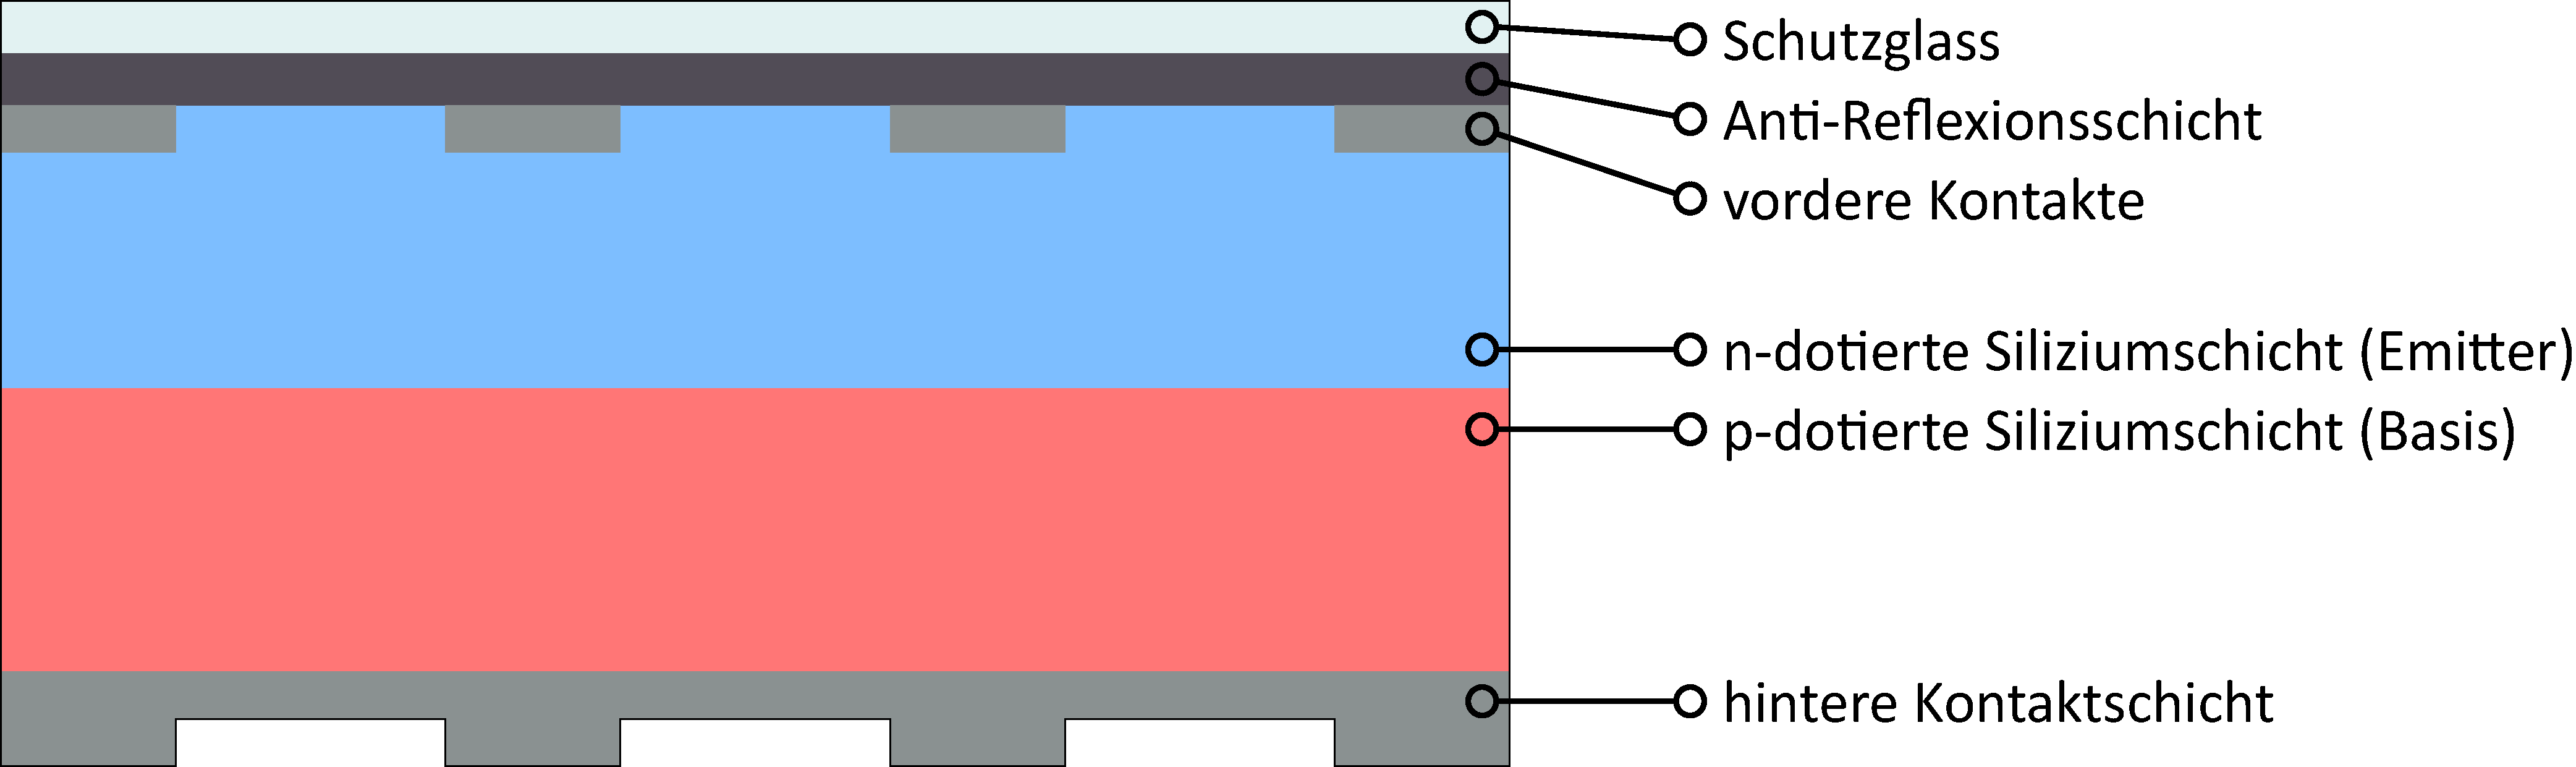
\includegraphics[width=1.0\linewidth]{solarzelle_schnitt.pdf}
        \caption{Grunlegender Aufbau einer Silizium-basierten Solarzelle}
    \end{figure}
    Die Dotierung der Schichten beschreibt einen Prozess bei dem ein
    Siliziumkristall mit Unreinheiten besetzt wird um dessen elektrische
    Leitfähigkeit zu beeinflussen. Silizium hat 4 Valenzelektronen und
    bildet somit Kristallstrukturen durch Kovalente Bindungen. Durch
    das dotieren mit Atomen mit mehr als 4 Valenzelektronen entsteht
    eine n-dotierte Schicht, bei dotieren mit Atomen mit weniger als 4
    Valenzelektronen eine p-dotierte Schicht.

\subsection{Funktionsweise}
    Wenn eine Solarzelle von Licht mit einer Wellenlängen von maximal
    1110nm getroffen wird welche nicht reflektiert werden, können diese
    bei Interaktion mit Atomen in den p- und n-dotierten Schichten
    Elektronen-Loch-Paare erzeugen.
    \begin{figure}[H]
        \centering
        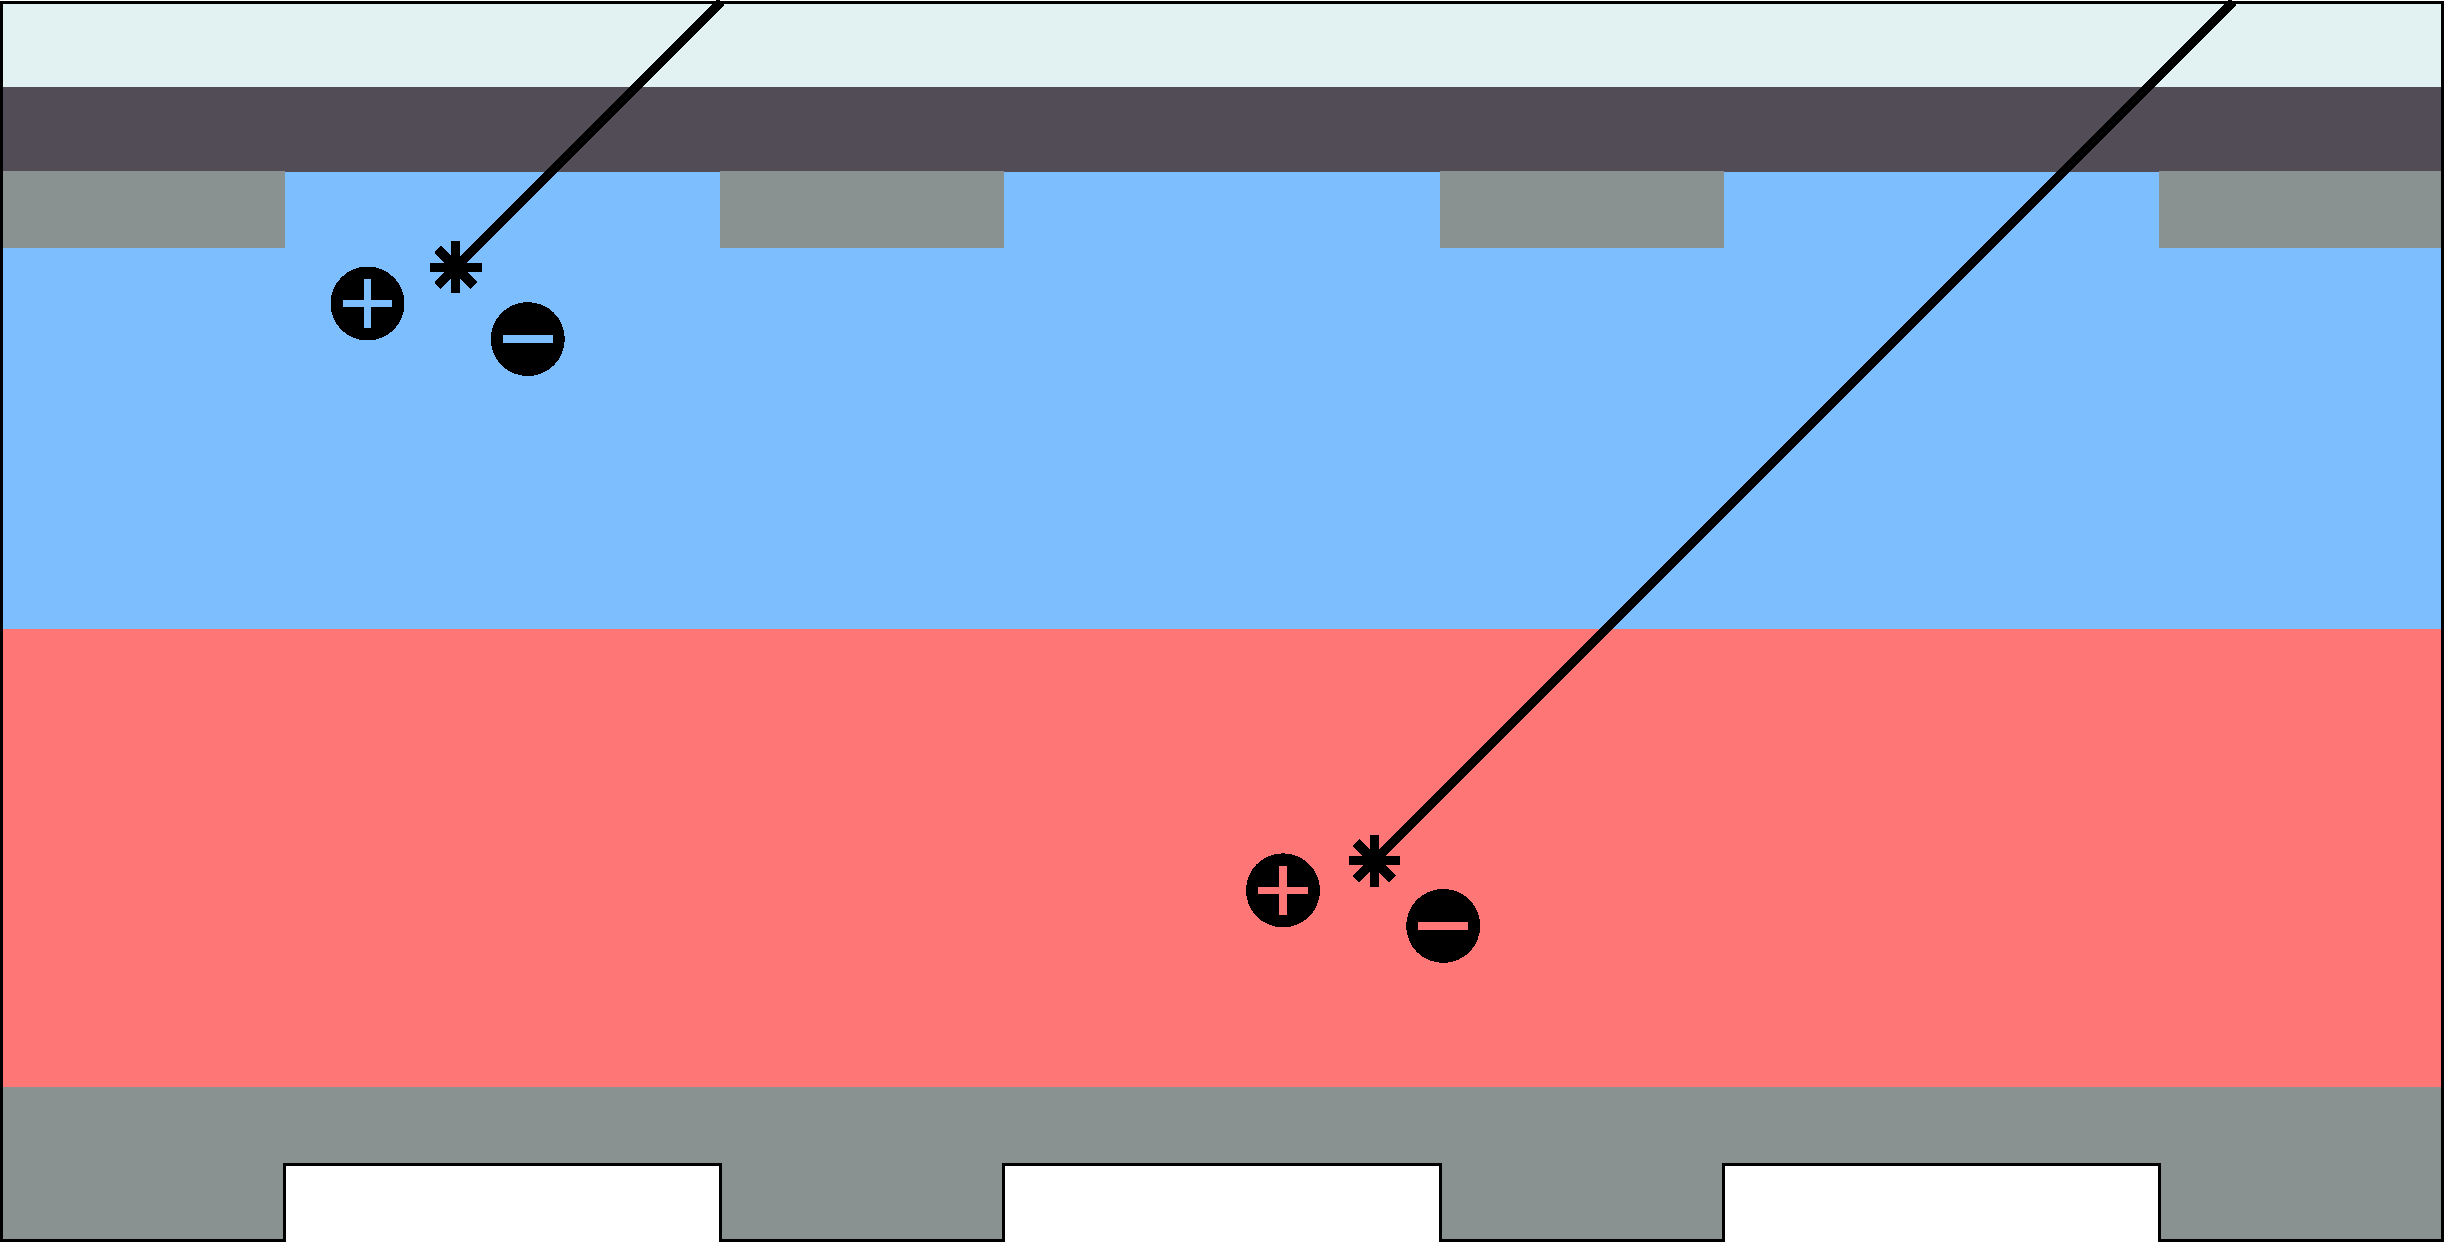
\includegraphics[width=0.65\linewidth]
        {solarzelle_schnitt_schritt1.pdf}
        \caption{Bildung von Elektronen-Loch-Paaren}
    \end{figure}

\newpage

    Durch den photovoltaischen Effekt bewegen sich die befreiten
    Elektronen in Richtung der der n-dotierten Schicht (blau) und
    Löcher in Richtung der p-dotierten Schicht (rot).
    \begin{figure}[H]
        \centering
        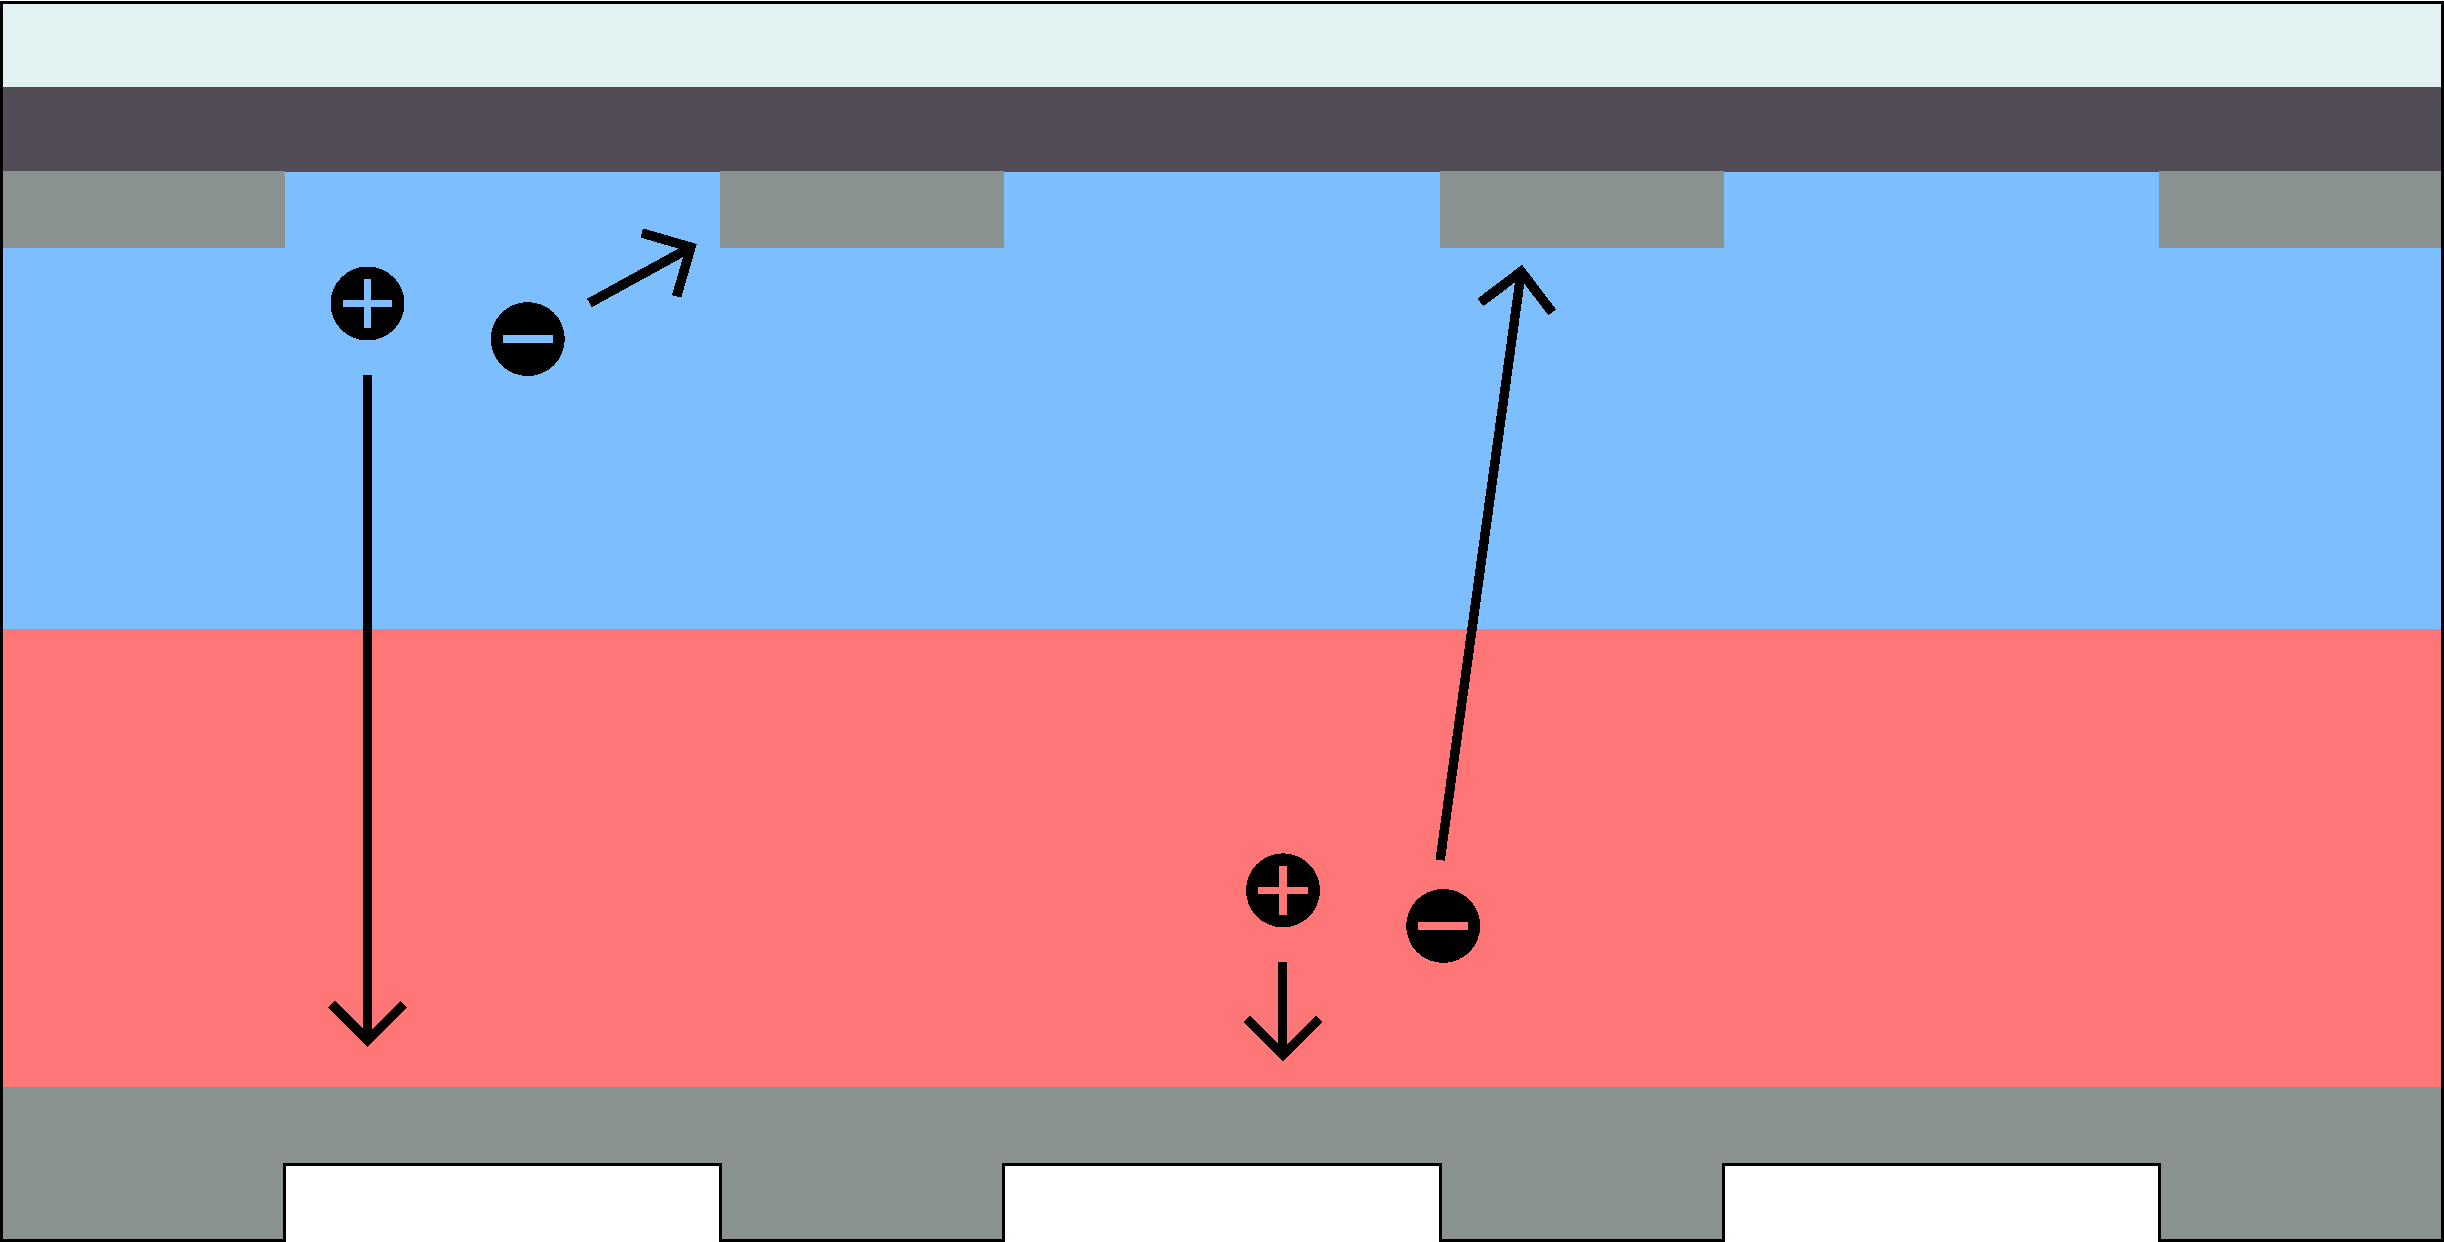
\includegraphics[width=0.65\linewidth]
        {solarzelle_schnitt_schritt2.pdf}
        \caption{Bildung des Photostroms}
    \end{figure}
    Der dabei entstehende Strom nennt sich Photostrom und die dabei
    Entstehende Potentialdifferenz erzeugt eine Spannung welche bei
    Anlegen eines externen Verbrauchers an die oberen und unteren
    Kontakte einen Messbaren Strom erzeugt.
    \begin{figure}[H]
        \centering
        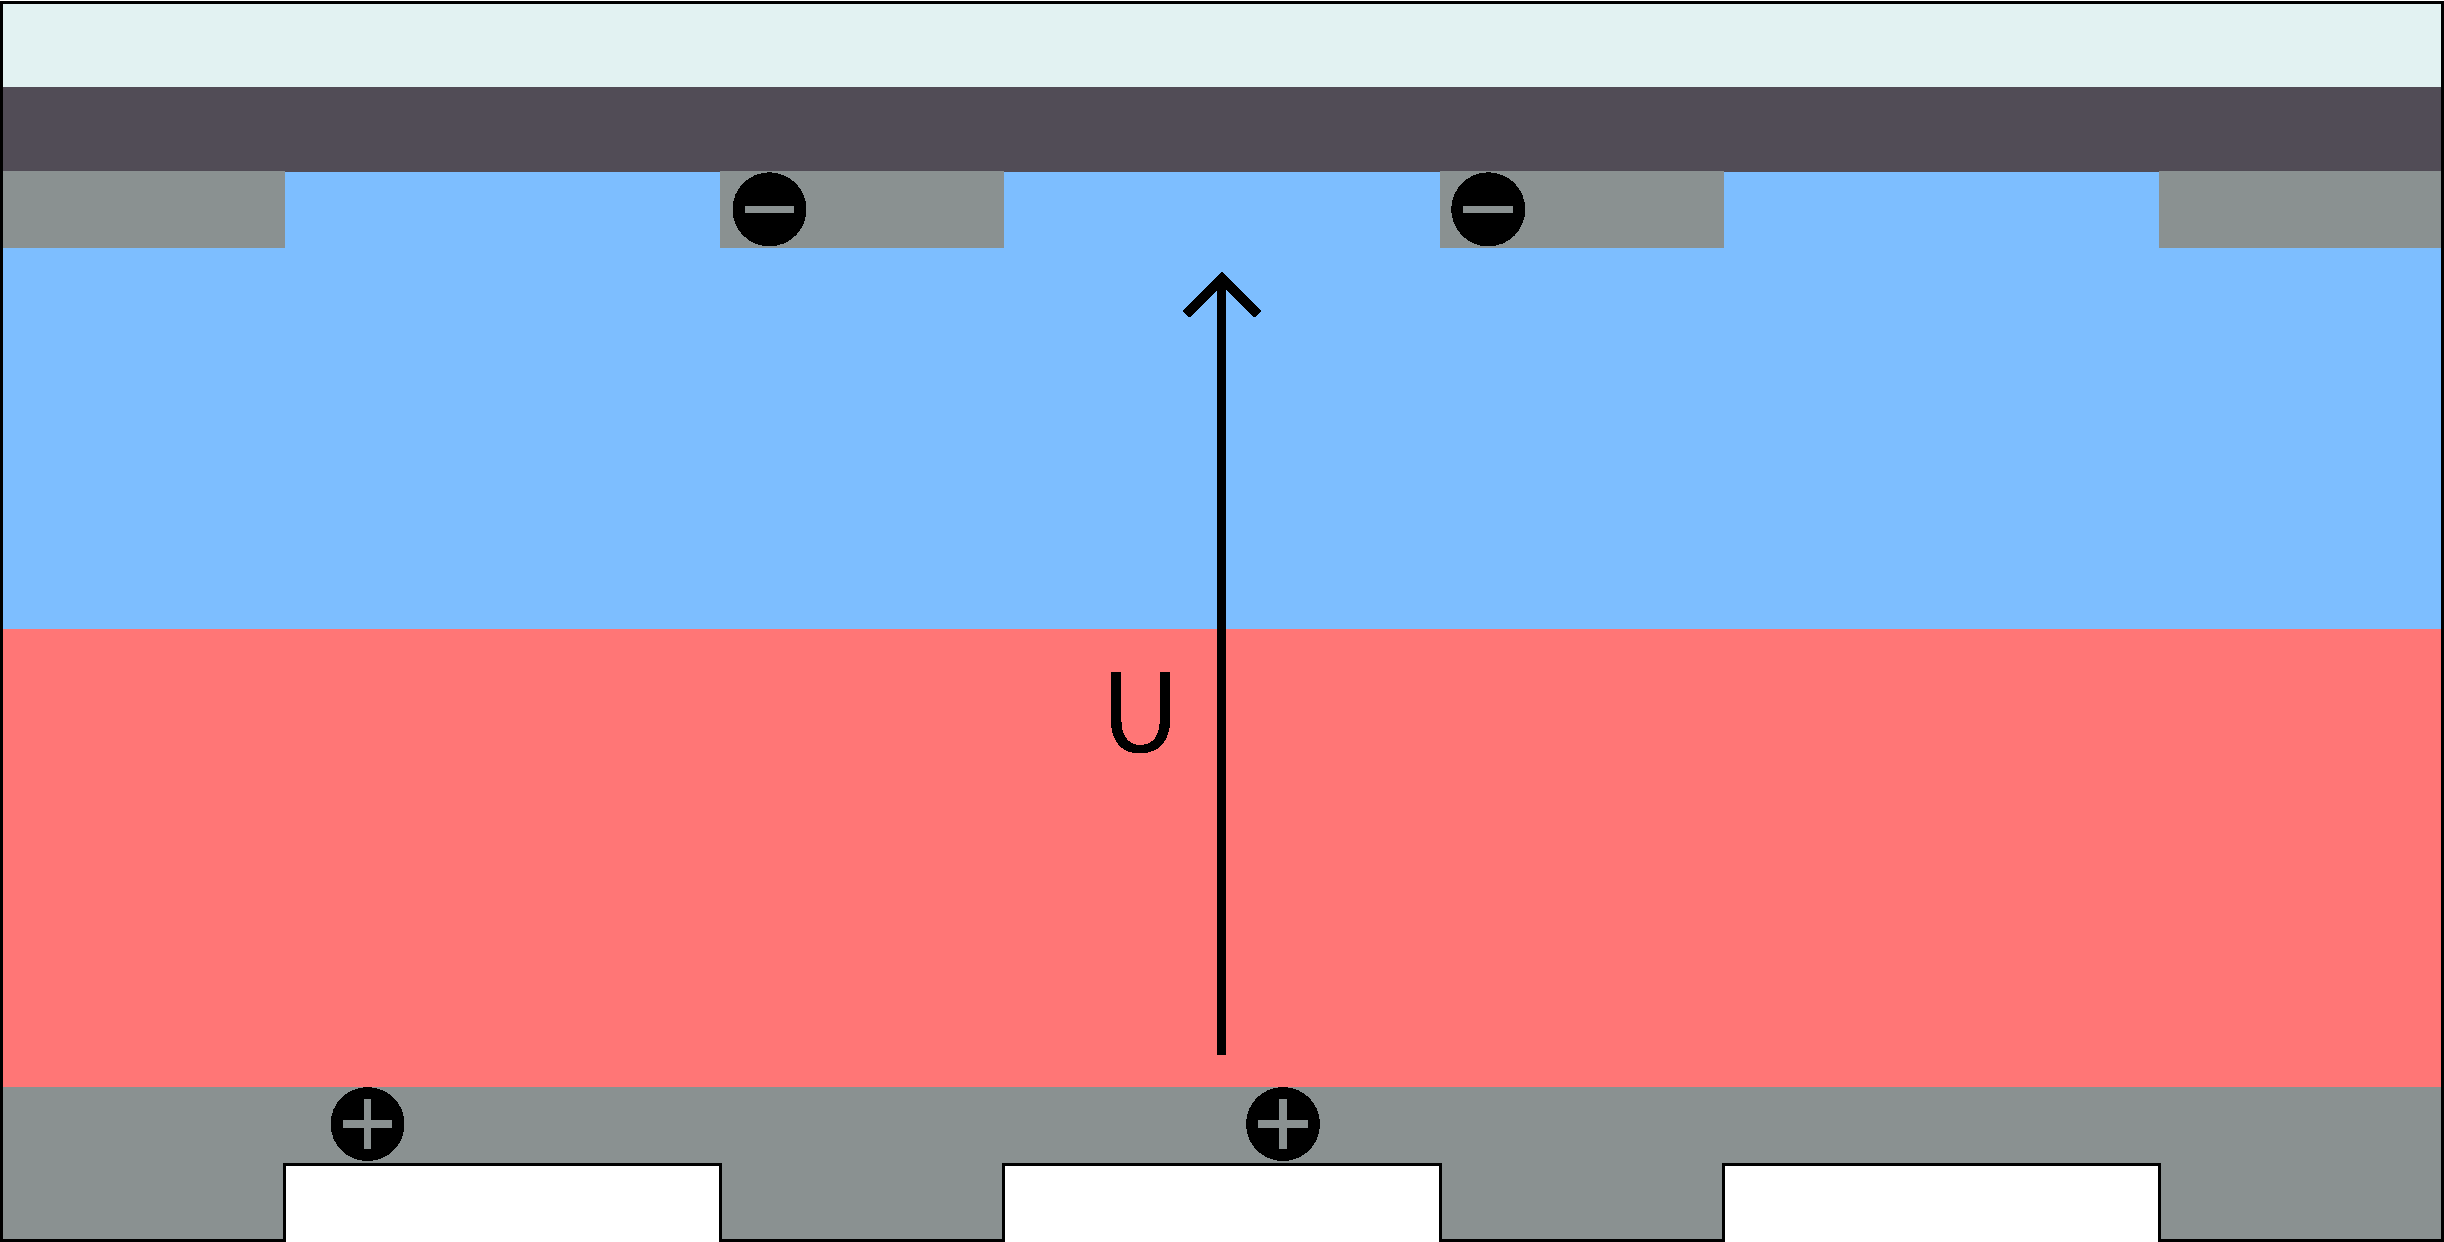
\includegraphics[width=0.65\linewidth]
        {solarzelle_schnitt_schritt3.pdf}
        \caption{Entstehen einer messbaren Spannung}
    \end{figure}
    Erst wenn ein externer Verbraucher angeschlossen ist, bewegen
    sich Elektronen und Löcher zu den nahe gelegenen Kontakten und
    dann über den Verbraucher zurück in die jeweiligen Sichten.

\subsection{Vorteile}
    Nach der Installation von Solarzellen wird kein Rohmaterial oder
    Energiezufluss benötigt um Energie zu sammeln. Dadurch dass
    Solarzellen keine beweglichen oder kontaktintensiven Teile besitzen
    brauchen sie beinahe keine Wartung und sind unanfällig gegenüber
    feuchten Witterungsverhältnissen \cite{SolarMaintenance}.\\
    Auch wenn Solarzellen wegen ihrer Umweltunfreundlichen Herstellung
    oft kritisiert werden, ist der Erntefaktor \footnote{Beschreibt das
    Verhältnis zwischen Erzeughter zu verbrauchter Energie} von
    Solarzellen etwa 26:1 (4\% Energieoffset) im vergleich zu den
    durchschnittlich 9:1 (11\% Energieoffset) von Kohle- und
    Ölkraftwerken \cite{SolarCarbonEmissions}.

\subsection{Nachteile}
    Solarzellen sind Anfällig für Temperaturschwankungen, bei
    höheren Temperaturen sinkt die Effizienz von Solarzellen. Die
    durschnittliche Energieeffizienz von Solarzellen liegt bei etwa
    15\% bis 20\% (unter Laborkonditionen) \cite{SolarEfficiency}, das
    heißt das rund 85\% bis 80\% der aufgefangenen Sonnenenergie
    entweder reflektiert oder in Wärme umgewandelt wird welche wiederum
    die Effizienz verringert (die überflüssige thermische Energie kann
    allerdings zur Effizienzsteigferung beitragen indem sie zur
    Versorgung von Kühlungsanlagen verwendet wird.
    \cite{YouTube_RE-SolarFlaw, PhotovoltaicPrinciples}.
    Solarzellen können nur am Tag Energie produzieren und ihre Effizienz
    sinkt in den Herbst- und Wintermonaten. Photovoltaische Zellen bieten
    nur dann eine ernstzunehmende Alternative für Nuklear-, Wind-, Hydro-
    oder sogar fossile Energie wenn die aufgesammelte Energie auch
    effizient gespeichert und transportiert werden kann.